\documentclass[aspectratio=1610]{beamer}

\usepackage{appendixnumberbeamer}
\usepackage[USenglish]{babel}
\usepackage[backend=bibtex,citestyle=authortitle]{biblatex}
\usepackage[scale=2]{ccicons}
\usepackage{color}
\usepackage{colortbl}
\usepackage{diagbox}
\usepackage{graphicx}
\usepackage{listings}
\usepackage{multicol}
\usepackage{pifont}
\usepackage{tikz}
\usetikzlibrary{positioning}
\usetikzlibrary{snakes}

\defbeamertemplate{section in toc}{numbered titles}{%
  \leavevmode
  \parbox[t]{1.5em}{\inserttocsectionnumber.}%
  \parbox[t]{\dimexpr\textwidth-1em\relax}{\inserttocsection}\par
}

\defbeamertemplate{subsection in toc}{indented titles}{%
  \leavevmode
  \parbox[t]{3em}{\hfill}%
  \parbox[t]{\dimexpr\textwidth-1em\relax}{\inserttocsubsection}\par
}

% this actually isn't totally hideous:
\usetheme[numbering=counter, progressbar=frametitle, sectionpage=none]{metropolis}
\setbeamertemplate{bibliography item}[text]
\setbeamertemplate{frametitle continuation}{}
\setbeamertemplate{section in toc}[numbered titles]
\setbeamertemplate{subsection in toc}[indented titles]

\title{Composable Concurrency Models}
\date{November 19, 2016}
\author{Dan Stelljes}

\bibliography{references}

\AtEveryBibitem{\clearfield{note}}
\AtEveryBibitem{\clearfield{url}}

\begin{document}
  \maketitle

  \section*{Introduction}

  \begin{frame}
    \centering
    \resizebox{0.8\linewidth}{!}{\begin{tikzpicture}
  \onslide<1->{
    \node at (0,0) {
      
\includegraphics[width=300pt]{browser}
    };
  }

  \onslide<2>{
    \path (-2.25,2.75) [draw=none, fill=darkgray, opacity=0.75] ellipse (60pt and 25pt);
    \node [text=white] at (-2.25,2.75) {
      Multiple tabs
    };

    \draw (2.25,2.25) [draw=none, fill=darkgray, opacity=0.75] ellipse (60pt and 25pt);
    \node [text=white] at (2.25,2.25) {
      Suggestions
    };

    \draw (0,0.5) [draw=none, fill=darkgray, opacity=0.75] ellipse (60pt and 25pt);
    \node [text=white] at (0,0.5) {
      Page rendering
    };

    \draw (-3,-1.5) [draw=none, fill=darkgray, opacity=0.75] ellipse (60pt and 25pt);
    \node [text=white] at (-3,-1.5) {
      Event handling
    };

    \draw (2.5,-1.5) [draw=none, fill=darkgray, opacity=0.75] ellipse (60pt and 25pt);
    \node [text=white] at (2.5,-1.5) {
      Background processes
    };
  }

  \onslide<3>{
    \node at (0,-0.62) {
      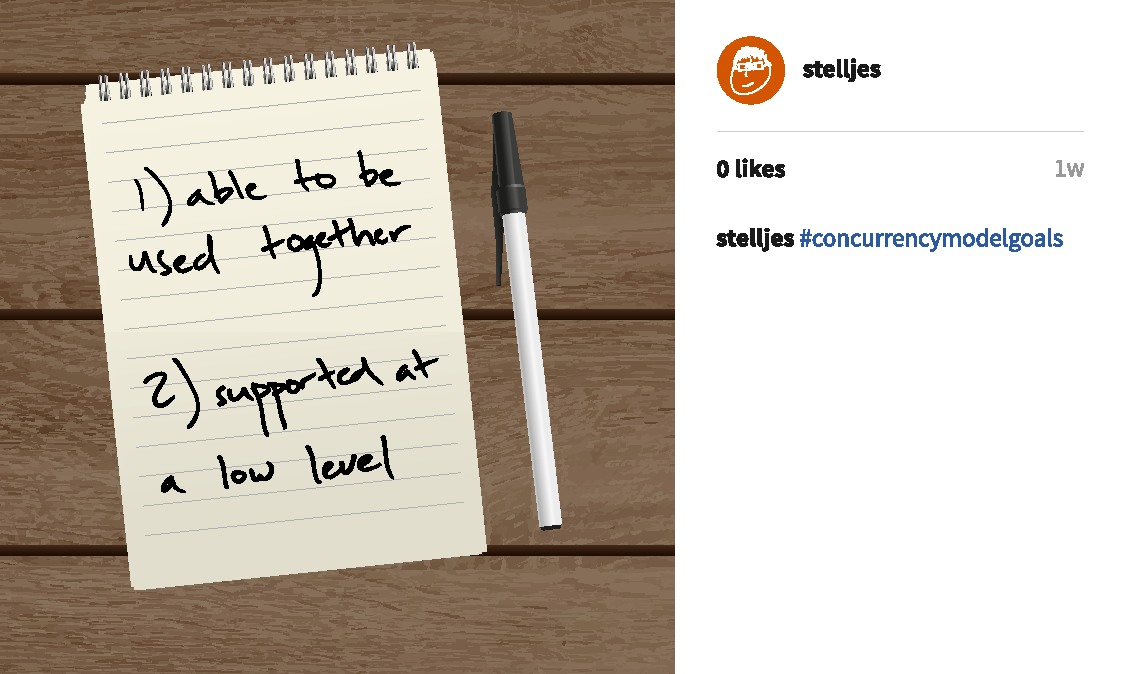
\includegraphics[width=220pt]{goals}
    };
  }
\end{tikzpicture}
}
  \end{frame}

  \begin{frame}
    \begin{multicols}{2}
      \tableofcontents
    \end{multicols}
  \end{frame}

  \section{Background}

  \subsection{Concurrency}

  \begin{frame}
    \frametitle{Threads and processes}

    \begin{figure}
      \centering
      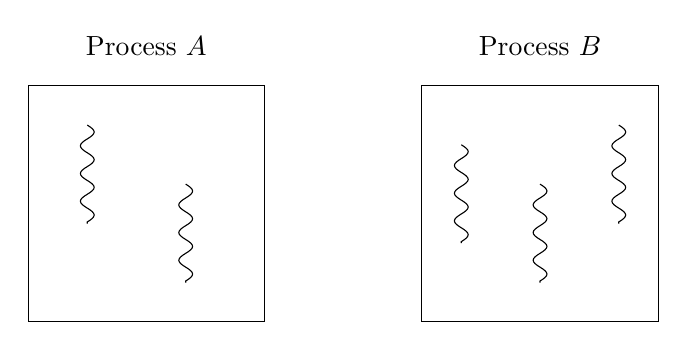
\begin{tikzpicture}
  \draw (-4,1.5) rectangle (-1,-1.5) node at (-2.5,2) { Process $A$ };
  \draw (1,1.5) rectangle (4,-1.5) node at (2.5,2) { Process $B$ };

  \draw[snake=coil,segment aspect=0] (-3.25,1) -- (-3.25,-0.25);
  \draw[snake=coil,segment aspect=0] (-2,0.25) -- (-2,-1);

  \draw[snake=coil,segment aspect=0] (1.5,0.75) -- (1.5,-0.5);
  \draw[snake=coil,segment aspect=0] (2.5,0.25) -- (2.5,-1);
  \draw[snake=coil,segment aspect=0] (3.5,1) -- (3.5,-0.25);
\end{tikzpicture}

    \end{figure}

    \vfill

    \begin{itemize}
      \item \textbf{Threads} are independent sequences of operations.
      \item \textbf{Processes} are instances of programs made up of one or more threads.
    \end{itemize}
  \end{frame}

  \begin{frame}
    \frametitle{Concurrency}

    \textbf{The ``happens before'' ($\rightarrow$) relation~\footcite{Lamport1977}}

    $A \rightarrow B$ if one of the following is true:

    \begin{enumerate}
      \item $A$ and $B$ are operations in the same thread and $A$ occurs before $B$.
      \item $A$ is the sending of a message by one thread and $B$ is the receipt of the same message by another thread.
    \end{enumerate}

    $A$ and $B$ are said to be concurrent if $A \nrightarrow B$ and $B \nrightarrow A$.
  \end{frame}

  \subsection{Complications}

  \begin{frame}
    \frametitle{Complications}

    \begin{itemize}
      \onslide<1->{
        \item \textbf{Sequential program:} Does the order of operations yield a correct result?
      }

      \vfill

      \onslide<2->{
        \item \textbf{Concurrent program:} Does \emph{every possible} order of operations yield a correct result?
      }
    \end{itemize}
  \end{frame}

  \begin{frame}
    \frametitle{Complications}
    \centering

    \textbf{Single thread:}
    \vfill
    \resizebox{0.9\linewidth}{!}{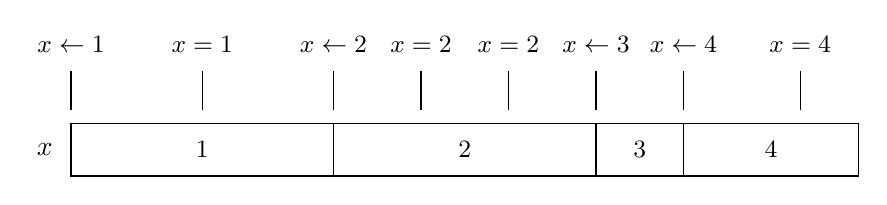
\begin{tikzpicture}
  \node at (-5.333,0) { $x$ };

  \draw (-5,-0.333) rectangle (-1.667,0.333) node [midway] { \small $1$ };
  \draw (-1.667,-0.333) rectangle (1.667,0.333) node [midway] { \small $2$ };
  \draw (1.667,-0.333) rectangle (2.778,0.333) node [midway] { \small $3$ };
  \draw (2.778,-0.333) rectangle (5,0.333) node [midway] { \small $4$ };

  \draw (-5,0.5) -- (-5,1) node [above=3pt] { \small $x \leftarrow 1$ };
  \draw (-3.333,0.5) -- (-3.333,1) node [above=3pt] { \small $x = 1$ };

  \draw (-1.667,0.5) -- (-1.667,1) node [above=3pt] { \small $x \leftarrow 2$ };
  \draw (-0.555,0.5) -- (-0.555,1) node [above=3pt] { \small $x = 2$ };
  \draw (0.555,0.5) -- (0.555,1) node [above=3pt] { \small $x = 2$ };

  \draw (1.667,0.5) -- (1.667,1) node [above=3pt] { \small $x \leftarrow 3$ };

  \draw (2.778,0.5) -- (2.778,1) node [above=3pt] { \small $x \leftarrow 4$ };
  \draw (4.26,0.5) -- (4.26,1) node [above=3pt] { \small $x = 4$ };
\end{tikzpicture}
}
  \end{frame}

  \begin{frame}
    \frametitle{Complications}
    \centering

    \textbf{Multiple threads:}
    \vfill
    \resizebox{0.9\linewidth}{!}{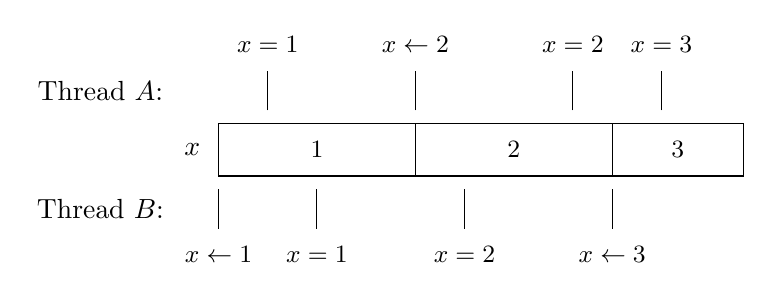
\begin{tikzpicture}
  \node at (-6.5,0.75) { Thread $A$: };
  \node at (-6.5,-0.75) { Thread $B$: };
  \node at (-5.333,0) { $x$ };

  \draw (-5,-0.333) rectangle (-2.5,0.333) node [midway] { \small $1$ };
  \draw (-2.5,-0.333) rectangle (0,0.333) node [midway] { \small $2$ };
  \draw (0,-0.333) rectangle (1.667,0.333) node [midway] { \small $3$ };

  \draw (-5,-0.5) -- (-5,-1) node [below=3pt] { \small $x \leftarrow 1$ };
  \draw (-4.375,0.5) -- (-4.375,1) node [above=3pt] { \small $x = 1$ };
  \draw (-3.75,-0.5) -- (-3.75,-1) node [below=3pt] { \small $x = 1$ };

  \draw (-2.5,0.5) -- (-2.5,1) node [above=3pt] { \small $x \leftarrow 2$ };
  \draw (-1.875,-0.5) -- (-1.875,-1) node [below=3pt] { \small $x = 2$ };
  \draw (-0.5,0.5) -- (-0.5,1) node [above=3pt] { \small $x = 2$ };

  \draw (0,-0.5) -- (0,-1) node [below=3pt] { \small $x \leftarrow 3$ };
  \draw (0.625,0.5) -- (0.625,1) node [above=3pt] { \small $x = 3$ };
\end{tikzpicture}
}
  \end{frame}

  \begin{frame}
    \frametitle{Complications}

    \centering
    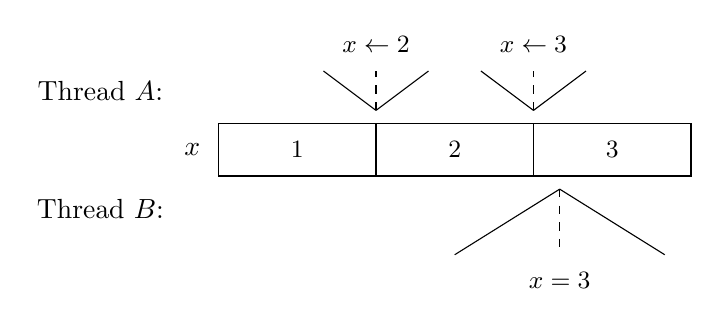
\begin{tikzpicture}
  \node at (-4.5,0.75) { Thread $A$: };
  \node at (-4.5,-0.75) { Thread $B$: };
  \node at (-3.333,0) { $x$ };

  \draw (-3,-0.333) rectangle (-1,0.333) node [midway] { \small $1$ };
  \draw (-1,-0.333) rectangle (1,0.333) node [midway] { \small $2$ };
  \draw (1,-0.333) rectangle (3,0.333) node [midway] { \small $3$ };

  \draw (-1.667,1) -- (-1,0.5) (-1,0.5) -- (-0.333,1);
  \draw [dashed] (-1,0.5) -- (-1,1) node [above=3pt] { \small $x \leftarrow 2$ };

  \draw (0.333,1) -- (1,0.5) (1,0.5) -- (1.667,1);
  \draw [dashed] (1,0.5) -- (1,1) node [above=3pt] { \small $x \leftarrow 3$ };

  \draw (0,-1.333) -- (1.333,-0.5) (1.333,-0.5) -- (2.667,-1.333);
  \draw [dashed] (1.333,-0.5) -- (1.333,-1.333) node [below=3pt] { \small $x = 3$ };
\end{tikzpicture}

  \end{frame}

  \subsection{Consistency models}

  \begin{frame}
    \frametitle{Linearizability}

    \begin{figure}
      \centering
      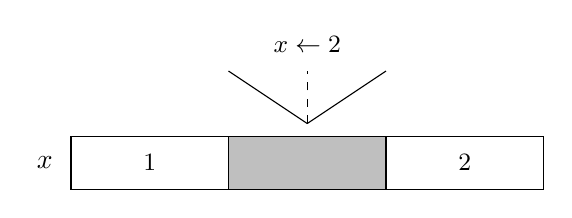
\begin{tikzpicture}
  \node at (-3.333,0) { $x$ };

  \draw (-3,-0.333) rectangle (-1,0.333) node [midway] { \small $1$ };
  \draw [fill=lightgray] (-1,-0.333) rectangle (1,0.333);
  \draw (1,-0.333) rectangle (3,0.333) node [midway] { \small $2$ };

  \draw (-1,1.167) -- (0,0.5) (0,0.5) -- (1,1.167);
  \draw [dashed] (0,0.5) -- (0,1.167) node [above=3pt] { \small $x \leftarrow 2$ };
\end{tikzpicture}

    \end{figure}

    \vfill

    \begin{itemize}
      \item Linearizability guarantees that the completion of an operation on a single object will appear to be instantaneous.
      \item The results of a linearizable operation will be visible as soon as the operation is complete.
    \end{itemize}
  \end{frame}

  \begin{frame}
    \frametitle{Serializability}

    \begin{figure}
      \centering
      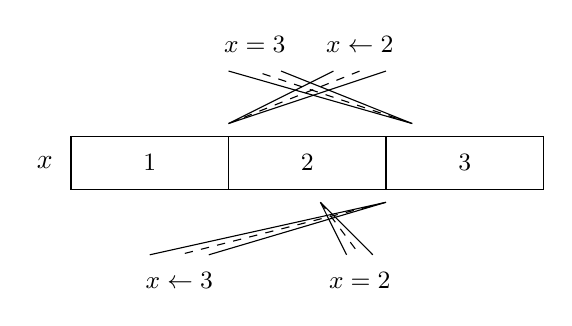
\begin{tikzpicture}
  \node at (-3.333,0) { $x$ };

  \draw (-3,-0.333) rectangle (-1,0.333) node [midway] { \small $1$ };
  \draw (-1,-0.333) rectangle (1,0.333) node [midway] { \small $2$ };
  \draw (1,-0.333) rectangle (3,0.333) node [midway] { \small $3$ };

  \draw (0.333,1.167) -- (-1,0.5) (-1,0.5) -- (1,1.167);
  \draw [dashed] (-1,0.5) -- (0.667,1.167) node [above=3pt] { \small $x \leftarrow 2$ };

  \draw (0.5,-1.167) -- (0.167,-0.5) (0.167,-0.5) -- (0.833,-1.167);
  \draw [dashed] (0.167,-0.5) -- (0.667,-1.167) node [below=3pt] { \small $x = 2$ };

  \draw (-2,-1.167) -- (1,-0.5) (1,-0.5) -- (-1.25,-1.167);
  \draw [dashed] (1,-0.5) -- (-1.625, -1.167) node [below=3pt] { \small $x \leftarrow 3$ };

  \draw (-1,1.167) -- (1.333,0.5) (1.333,0.5) -- (-0.333,1.167);
  \draw [dashed] (1.333,0.5) -- (-0.667,1.167) node [above=3pt] { \small $x = 3$ };
\end{tikzpicture}

    \end{figure}

    \vfill

    \begin{itemize}
      \item Serializability guarantees that operations can occur in any order as long as an equivalent sequential ordering exists.
      \item While a serializable set of operations is being executed, it appears to be the only set of operations being executed.
    \end{itemize}
  \end{frame}

  \begin{frame}
    \frametitle{Strict serializability}

    \begin{itemize}
      \item Linearizability \emph{and} serializability yield strict serializability, which guarantees both consistency and isolation.
    \end{itemize}

    \vfill

    \textbf{Strict serializability~\footcite{Herlihy1990}}

    An ordering of operations is equivalent to some sequential ordering and that ordering corresponds to the order of execution in real time.
  \end{frame}

  \addtocontents{toc}{\hfill}

  \section{Concurrency models}

  \subsection{Atomic variables}

  \begin{frame}
    \frametitle{Atomic variables}

    \begin{columns}
      \begin{column}{0.5\textwidth}
        \centering
        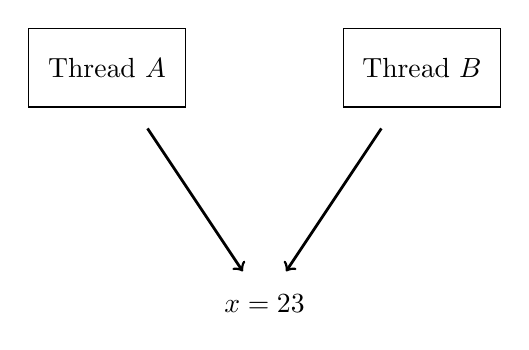
\begin{tikzpicture}
  \node at (0,-3) (x) { $x = 23$ };

  \draw (-3,0.5) rectangle (-1,-0.5) node [midway] (A) { Thread $A$ };
  \draw (1,0.5) rectangle (3,-0.5) node [midway] (B) { Thread $B$ };

  \draw[->, line width=1pt, shorten <=18pt, shorten >=6pt] (A) -- (x);
  \draw[->, line width=1pt, shorten <=18pt, shorten >=6pt] (B) -- (x);
\end{tikzpicture}

      \end{column}
      \hfill
      \begin{column}{0.5\textwidth}
        $x = 23$

        \begin{enumerate}
          \item $A$ reads $x$
          \item $B$ reads $x$
          \item $A$ increments value
          \item $A$ writes incremented value to $x$
          \item $B$ increments value
          \item $B$ writes incremented value to $x$
        \end{enumerate}

        $x = 24$
      \end{column}
    \end{columns}
  \end{frame}

  \begin{frame}
    \frametitle{Atomic variables}

    \begin{columns}
      \begin{column}{0.5\textwidth}
        \centering
        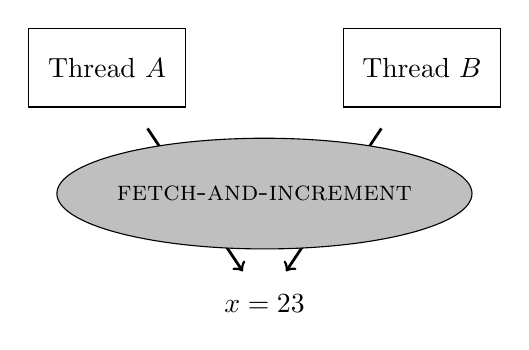
\begin{tikzpicture}
  \node at (0,-3) (x) { $x = 23$ };

  \draw (-3,0.5) rectangle (-1,-0.5) node [midway] (A) { Thread $A$ };
  \draw (1,0.5) rectangle (3,-0.5) node [midway] (B) { Thread $B$ };

  \draw[->, line width=1pt, shorten <=18pt, shorten >=6pt] (A) -- (x);
  \draw[->, line width=1pt, shorten <=18pt, shorten >=6pt] (B) -- (x);

  \draw [fill=lightgray] (0,-1.6) ellipse (75pt and 20pt) node at (0, -1.6) { \textsc{fetch-and-increment} };
\end{tikzpicture}

      \end{column}
      \hfill
      \begin{column}{0.5\textwidth}
        $x = 23$

        \begin{enumerate}
          \item $A$ calls \textsc{fetch-and-increment} on $x$
          \item $B$ calls \textsc{fetch-and-increment} on $x$
        \end{enumerate}

        $x = 25$
      \end{column}
    \end{columns}
  \end{frame}

  \begin{frame}
    \frametitle{Atomic variables}
    \centering
    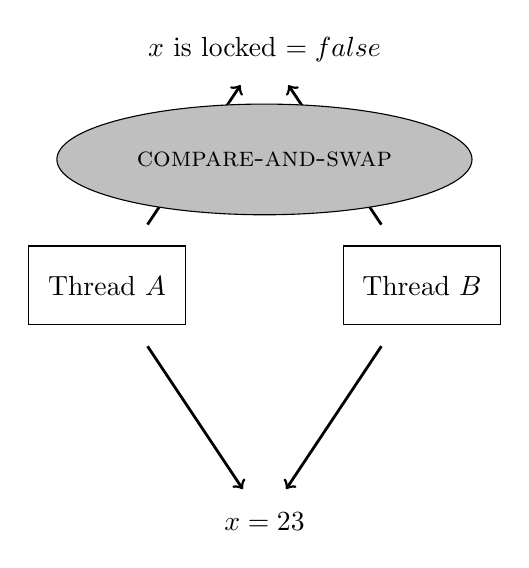
\begin{tikzpicture}
  \node at (0,3) (lock) { $x$ is locked $= false$ };
  \node at (0,-3) (x) { $x = 23$ };

  \draw (-3,0.5) rectangle (-1,-0.5) node [midway] (A) { Thread $A$ };
  \draw (1,0.5) rectangle (3,-0.5) node [midway] (B) { Thread $B$ };

  \draw[->, line width=1pt, shorten <=18pt, shorten >=6pt] (A) -- (lock);
  \draw[->, line width=1pt, shorten <=18pt, shorten >=6pt] (B) -- (lock);

  \draw[->, line width=1pt, shorten <=18pt, shorten >=6pt] (A) -- (x);
  \draw[->, line width=1pt, shorten <=18pt, shorten >=6pt] (B) -- (x);

  \draw [fill=lightgray] (0,1.6) ellipse (75pt and 20pt) node at (0, 1.6) { \textsc{compare-and-swap} };
\end{tikzpicture}

  \end{frame}

  \begin{frame}
    \frametitle{Atomic variables}
    \centering
    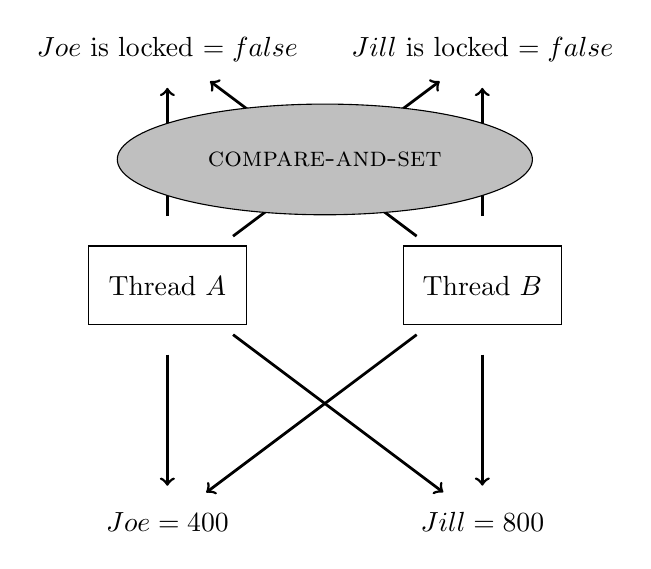
\begin{tikzpicture}
  \node at (-2,3) (joe-lock) { $Joe$ is locked $= false$ };
  \node at (2,3) (jill-lock) { $Jill$ is locked $= false$ };

  \node at (-2,-3) (joe) { $Joe = 400$ };
  \node at (2,-3) (jill) { $Jill = 800$ };

  \draw (-3,0.5) rectangle (-1,-0.5) node [midway] (A) { Thread $A$ };
  \draw (1,0.5) rectangle (3,-0.5) node [midway] (B) { Thread $B$ };

  \draw[->, line width=1pt, shorten <=18pt, shorten >=6pt] (A) -- (joe-lock);
  \draw[->, line width=1pt, shorten <=18pt, shorten >=6pt] (B) -- (joe-lock);

  \draw[->, line width=1pt, shorten <=18pt, shorten >=6pt] (A) -- (joe);
  \draw[->, line width=1pt, shorten <=18pt, shorten >=6pt] (B) -- (joe);

  \draw[->, line width=1pt, shorten <=18pt, shorten >=6pt] (A) -- (jill-lock);
  \draw[->, line width=1pt, shorten <=18pt, shorten >=6pt] (B) -- (jill-lock);

  \draw[->, line width=1pt, shorten <=18pt, shorten >=6pt] (A) -- (jill);
  \draw[->, line width=1pt, shorten <=18pt, shorten >=6pt] (B) -- (jill);

  \draw [fill=lightgray] (0,1.6) ellipse (75pt and 20pt) node at (0, 1.6) { \textsc{compare-and-set} };
\end{tikzpicture}

  \end{frame}

  \subsection{Software transactional memory}

  \begin{frame}
    \frametitle{Software transactional memory}

    Software transactional memory (STM) is an optimistic approach to working with shared memory:~\footcite{Shavit1995}

    \begin{enumerate}
      \item A thread writes to a shared memory location, keeping track of the transaction in a log.
      \item If there are conflicting changes at the end of the transaction, the transaction is aborted and retried.
      \item If there are no conflicts, the changes are committed and become visible.
    \end{enumerate}
  \end{frame}

  \begin{frame}
    \frametitle{Software transactional memory}
    \centering
    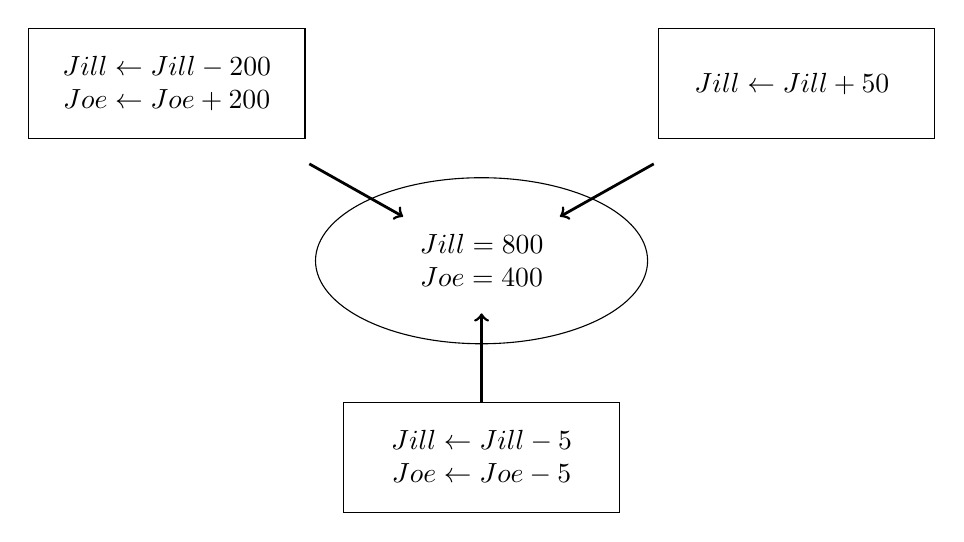
\begin{tikzpicture}
  \draw (0,0) ellipse (60pt and 30pt) node [align=center,midway] (accounts) {
    $Jill = 800$\\$Joe = 400$
  };

  \node at (-4,2.25) [align=center,draw,minimum height=40pt,minimum width=100pt] (A) {
    $Jill \leftarrow Jill - 200$\\$Joe \leftarrow Joe + 200$
  };

  \node at (4,2.25) [align=center,draw,minimum height=40pt,minimum width=100pt] (B) {
    $Jill \leftarrow Jill + 50$
  };

  \node at (0,-2.5) [align=center,draw,minimum height=40pt,minimum width=100pt] (C) {
    $Jill \leftarrow Jill - 5$\\
    $Joe \leftarrow Joe - 5$
  };

  \draw[->, line width=1pt, shorten <=18pt, shorten >=6pt] (A) -- (accounts);
  \draw[->, line width=1pt, shorten <=18pt, shorten >=6pt] (B) -- (accounts);
  \draw[->, line width=1pt, shorten >=6pt] (C) -- (accounts);
\end{tikzpicture}

  \end{frame}

  \subsection{Communicating threads}

  \begin{frame}
    \frametitle{Communicating threads}
    \centering
    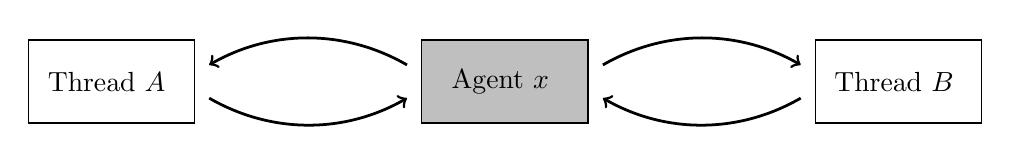
\begin{tikzpicture}
  \node at (-5,0) [align=center,draw,minimum height=30pt,minimum width=60pt] (A) {
    Thread $A$
  };

  \node at (0,0) [align=center,draw,fill=lightgray,minimum height=30pt,minimum width=60pt] (x) {
    Agent $x$
  };

  \node at (5,0) [align=center,draw,minimum height=30pt,minimum width=60pt] (B) {
    Thread $B$
  };

  \path[<-,line width=1pt, shorten <=6pt, shorten >=6pt] ([yshift=3pt]A.east) edge[in=150,out=30] ([yshift=3pt]x.west);
  \path[->,line width=1pt, shorten <=6pt, shorten >=6pt] ([yshift=-3pt]A.east) edge[in=-150,out=-30] ([yshift=-3pt]x.west);

  \path[<-,line width=1pt, shorten <=6pt, shorten >=6pt] ([yshift=3pt]B.west) edge[in=30,out=150] ([yshift=3pt]x.east);
  \path[->,line width=1pt, shorten <=6pt, shorten >=6pt] ([yshift=-3pt]B.west) edge[in=-30,out=-150] ([yshift=-3pt]x.east);
\end{tikzpicture}

    \vfill
    \textbf{Agents:} An isolated thread wraps an object.~\footcite{Swalens2014}
  \end{frame}

  \begin{frame}
    \frametitle{Communicating threads}
    \centering
    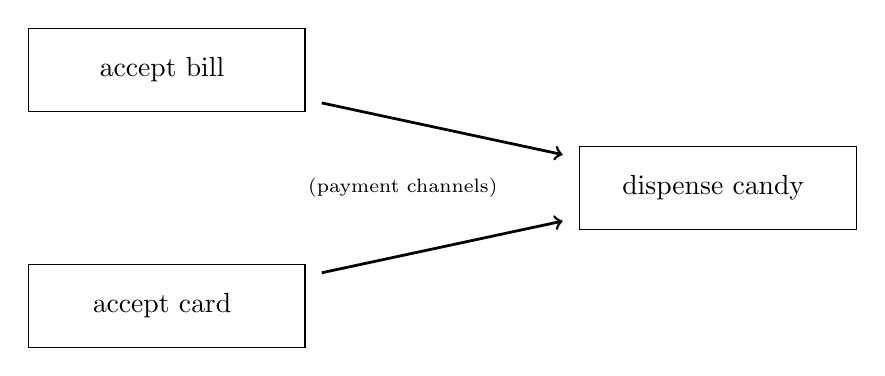
\begin{tikzpicture}
  \node at (-4,1.5) [align=center,draw,minimum height=30pt,minimum width=100pt] (bill) {
    accept bill
  };

  \node at (-4,-1.5) [align=center,draw,minimum height=30pt,minimum width=100pt] (card) {
    accept card
  };

  \node at (3,0) [align=center,draw,minimum height=30pt,minimum width=100pt] (dispense) {
    dispense candy
  };

  \node at (-1,0) (channels) {
    \scriptsize (payment channels)
  };

  \draw[->,line width=1pt, shorten <=6pt, shorten >=6pt] (bill) -- (dispense);
  \draw[->,line width=1pt, shorten <=6pt, shorten >=6pt] (card) -- (dispense);
\end{tikzpicture}

    \vfill
    \textbf{Communicating sequential processes (CSP):} Independent threads communicate synchronously through predefined channels.~\footcite{Hoare1978}
  \end{frame}

  \begin{frame}
    \frametitle{Communicating threads}
    \centering
    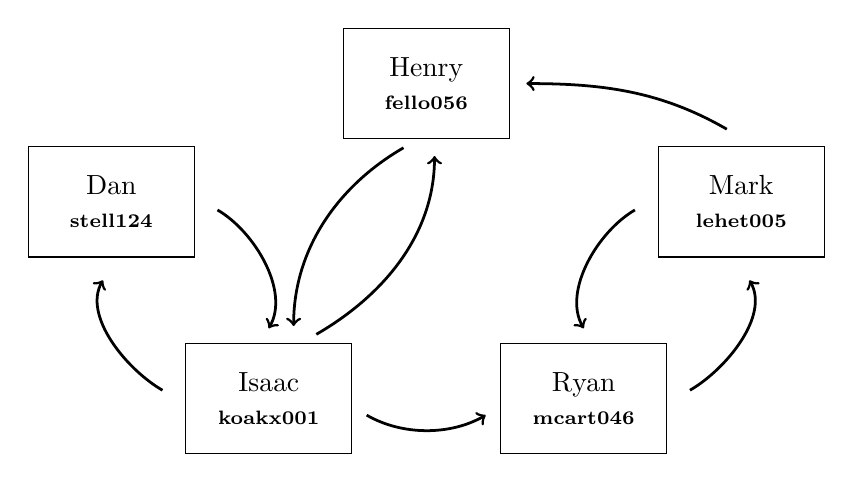
\begin{tikzpicture}
  \node at (-4,1.5) [align=center,draw,minimum height=40pt,minimum width=60pt] (dan) {
    Dan\\
    \scriptsize\textbf{stell124}
  };

  \node at (0,3) [align=center,draw,minimum height=40pt,minimum width=60pt] (henry) {
    Henry\\
    \scriptsize\textbf{fello056}
  };

  \node at (4,1.5) [align=center,draw,minimum height=40pt,minimum width=60pt] (mark) {
    Mark\\
    \scriptsize\textbf{lehet005}
  };

  \node at (-2,-1) [align=center,draw,minimum height=40pt,minimum width=60pt] (isaac) {
    Isaac\\
    \scriptsize\textbf{koakx001}
  };

  \node at (2,-1) [align=center,draw,minimum height=40pt,minimum width=60pt] (ryan) {
    Ryan\\
    \scriptsize\textbf{mcart046}
  };

  \path[->,line width=1pt, shorten <=6pt, shorten >=6pt] ([xshift=3pt]dan.east) edge[in=60,out=-30] ([xshift=-3pt]isaac.north);
  \path[->,line width=1pt, shorten <=6pt, shorten >=6pt] ([xshift=-3pt]isaac.west) edge[in=240,out=150] ([yshift=-3pt]dan.south);

  \path[->,line width=1pt, shorten <=6pt, shorten >=6pt] ([xshift=12pt]isaac.north) edge[in=270,out=30] ([xshift=3pt]henry.south);
  \path[->,line width=1pt, shorten <=6pt, shorten >=6pt] ([xshift=-3pt]henry.south) edge[in=90,out=210] ([xshift=9pt]isaac.north);

  \path[->,line width=1pt, shorten <=6pt, shorten >=6pt] ([yshift=-3pt]isaac.east) edge[in=210,out=-30] ([yshift=-3pt]ryan.west);

  \path[->,line width=1pt, shorten <=6pt, shorten >=6pt] ([xshift=-3pt]mark.west) edge[in=120,out=210] ([xshift=3pt]ryan.north);
  \path[->,line width=1pt, shorten <=6pt, shorten >=6pt] ([xshift=3pt]ryan.east) edge[in=300,out=30] ([yshift=-3pt]mark.south);

  \path[->,line width=1pt, shorten <=6pt, shorten >=6pt] ([yshift=3pt]mark.north) edge[in=0,out=150] (henry.east);
\end{tikzpicture}

    \vfill
    \textbf{The actor model:} Independent threads send messages to known addresses.~\footcite{Agha1986}
  \end{frame}

  % never change, LaTeX
  \addtocontents{toc}{\newpage}

  \section{Composability}

  \subsection{Correctness criteria}

  \begin{frame}
    \frametitle{Correctness criteria}

    \textbf{How do we know that models are composable?~\footcite{Swalens2014}}

    \begin{itemize}
      \item Safety: ``Nothing bad will happen!'' (The output of a program or algorithm will not be incorrect.)
      \item Liveness: ``Something will eventually happen!'' (The program or algorithm will terminate.)
    \end{itemize}

    Two models are composable if using them within each other doesn't compromise safety or liveness.
  \end{frame}

  \subsection{Possible conflicts}

  \begin{frame}
    \frametitle{Possible conflicts}
    \small

    \newcommand{\n}{\textcolor{red}{\ding{55}}}
    \newcommand{\y}{\textcolor{olive}{\ding{51}}}

    \vfill
    \begin{tabular}{c | c c c c | c c c c}
      & \multicolumn{4}{c|}{\textbf{Safety}} & \multicolumn{4}{|c}{\textbf{Liveness}} \tabularnewline
      \diagbox[dir=NW,width=7em]{within}{using} & atoms & refs & agents & channels & atoms & refs & agents & channels \tabularnewline
      \hline
      atoms & \n & \n & \n & \n & \y & \y & \y & \n \tabularnewline
      refs & \n & \y & \y & \n & \y & \y & \y & \n \tabularnewline
      agents & \y & \y & \y & \y & \y & \y & \y & \n \tabularnewline
      channels & \y & \y & \y & \y & \y & \y & \n & \n \tabularnewline
    \end{tabular}
    \vfill
    \begin{itemize}
      \onslide<2->{
        \item A model reexecutes code that performs an irrevocable action.
      }
      \onslide<3->{
        \item A model reexecutes code that causes the reexecution to continually happen.
      }
      \onslide<4->{
        \item A model that supports blocking operations is used within a model that doesn't.
      }
      \onslide<5->{
        \item A model does not guarantee safety or liveness by design.
      }
    \end{itemize}
  \end{frame}

  \subsection{Ongoing work}

  \begin{frame}
    \frametitle{Ongoing work}

    \begin{itemize}
      \onslide<1->{
        \item Composable ``building blocks'' (thread creation, message passing, etc.) that could be used to build common concurrency models~\footcite{Swalens2014}
      }
      \vfill
      \onslide<2->{
        \item Unifying abstractions for high-level language virtual machines~\footcite{Marr2012}
      }
      \vfill
      \onslide<3->{
        \item Formal theories for safely composing concurrency control~\footcite{Ziv2015}
      }
    \end{itemize}
  \end{frame}

  \begin{frame}[standout]
    \centering
    Thanks to Elena Machkasova, K.K. Lamberty, and Matthew Justin for their guidance and suggestions.
    \vfill
    \href{https://github.com/dstelljes/senior-sem}{github.com/dstelljes/senior-sem}
    \vfill
    \ccbyncsa{}
  \end{frame}

  \appendix{}

  \begin{frame}[allowframebreaks]
    \frametitle{References}

    \printbibliography{}
  \end{frame}

\end{document}
